\chapter{引言}\label{chap:introduction}

\section{目的与意义}

随着集成电路晶体管数量的不断增加,能够有更多的资源来支持更为复杂但效率更高的处理器微结构特性,包括了乱序调度,超标量发射和指令缓存。得益于这些复杂的特性,微处理器能够从五级流水的性能瓶颈中解放出来,在存储墙愈加严重的现状下依然能够得到性能的提升。自主设计出一款乱序双发射处理器正是出于对计算性能提高的不懈追求。同时,在设计、调试、评测、分析、优化的过程中能够积累高性能通用处理器设计的宝贵经验。

和静态流水线相对固定的格式不同,乱序多发射的处理器在设计中更加灵活。很多方案、参数糅合在一起复杂地影响着处理器的性能,需要比较、权衡与取舍。对处理器设计空间的初步探索,同样具有意义。

\section{研究背景}

近年来,RISC-V开源体系结构的兴起,使得很多软硬件实力相对于大公司薄弱很多的研究个体受益良多。RISC-V开源的项目越来越多,其中有微处理器的设计实现如Rocket和BOOM;有更抽象的电路描述语言如Chisel;也有RISC-V的指令模拟器如Spike,可以在上面调试软件,或者得到程序的执行写回信息用来调试处理器;还有已经移植完成的上层应用软件栈如Linux,GCC和LLVM。这些开源的项目大大降低了研究个体独立设计出一款高性能处理器以及在上面运行软件栈的难度与门槛。

从指令集ISA,编程语言,开源项目三个角度来看,RISC-V开源体系结构对毕业设计都有很多的助益。

\subsection{MIPS和RISC-V}\label{subsec:ISA}
设计一款具体的CPU要对应于具体的ISA,这里有两个较为简单的指令集可供选择:一个是MIPS的MIPS32子集,一个是RISC-V的RV32I子集,两者都是RISC的典型ISA。MIPS体系结构从最开始1985年推出的第一代指令集MIPS I和R2000处理器起,已经有三十多年的历史;而RISC-V作为加州大学伯克利分校的RISC系列的第五代指令集,在其师生大力推广下成为了近年来热度最高的开源指令集。

设计中最后选择RV32I而不是MIPS32有多方面的考虑。首先是出于对新事物的好奇和新鲜感;其次由于本科的教学的参考ISA是MIPS,通过本科的学习和工程实践对于MIPS的有了初步的认识,也能够体察到MIPS在ISA设计中的一些缺陷:
\begin{enumerate}[label=(\alph*)]
	\item 延迟槽的引入,这个当初对单发射五级流水从体系结构上做出的优化被日后的工程实践证明是一个历史的包袱。因为分支指令后面紧跟一条延迟槽的设计仅仅适用于像单发射五级静态流水这样的简单的设计中。超标量、乱序投机取指的高性能处理器取指仍然需要做转移猜测,所以延迟槽的引入反而增加了高性能处理器取指和中断例外设计的复杂度。
	\item 为了存储定点乘除法结果而单独加入了HILO寄存器,再通过MFHI, HFLO, MTHI, MTLO这四条指令与通用寄存器堆进行相互搬运也会增加处理器设计的复杂度。
	\item 继续深入分析,MIPS的特权态的设计显得很凌乱,对于特权模式的处理机制是逐渐增量式添加的方式,并不是一开始就规划地非常清楚,欠缺体系。
	\item 在80年代MIPS诞生之初也没有考虑到64位虚拟地址空间的需求和嵌入式领域指令压缩的需求,导致指令空间设计考虑不周,64位尚能够与32位兼容,但是为嵌入式压缩指令引入的microMIPS就是重新设计的与原有的MIPS 32/64并不兼容的另一套ISA。而且由于延迟槽的存在,压缩的效果也不及ARM的Thumb-2和RISC-V的RV32I+RVC。对比不同压缩指令集编译出来的统一程序的二进制代码大小如图\ref{fig:sizecmp}所示:
	\begin{figure}[!htbp]
		\centering
		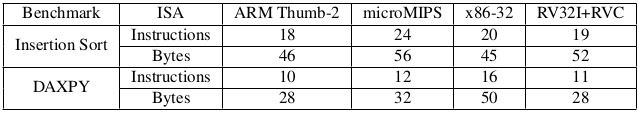
\includegraphics[width=0.8\linewidth]{ISA_Size_cmp.png}
		\bicaption{不同压缩指令集编译插入排序和双精度浮点乘加程序的代码大小比较。\citep{Patterson:2017:RRO:3202479}图 7.2.}{Instructions and code size for Insertion Sort and DAXPY for compressed ISAs. Figure 7.2 of \citep{Patterson:2017:RRO:3202479}.}
		\label{fig:sizecmp}
	\end{figure}
\end{enumerate}

ISA体系结构的演进发展已经有50多年的历史了,在诸如上述设计教训的沉淀下,最为基础核心的设计趋向于收敛。所以比MIPS晚诞生20多年的RISC-V能够站在后来者的角度审视之前诞生的众多指令集的优缺点,从设计开始就有一套清晰的规划,摒弃了很多包括上文提及的MIPS指令集设计中的缺陷,做到32位,64位,压缩变长指令集很好的统一,以简洁规整的形式呈现出来,最大化的简化了硬件指令译码的逻辑。同时,因为有了系统的规划,虽然目前特权态的有些规定还不是很明确,高性能的SIMD指令亦或是向量指令也不完善,但是对于处理器运行的模式规划确实非常明确有章法。另外,指令编码空间设计合理使得指令的可拓展性极强,以便日后之需。下面通过对比MIPS来具体分析RISC-V的特点以及简洁优美的设计考虑。

首先不同于几乎所有的先前的ISA,RISC-V是模块化的。核心是基础的ISA --- RV32I,简单而不失强大,足以运行整个软件栈。同时,RV32I是被冻结,也即永远不会改变,是稳定的,这样,对硬件设计人员或者软件设计人员都友好。其他的扩展功能的指令以可选的方式添加,比如也已经被冻结的RV64I基础系列和M(乘除法)、A(原子指令)、F(单精度浮点)、D(双精度浮点)等拓展系列\citep{Patterson:2017:RRO:3202479}。
\begin{enumerate}%[label=( \arabic* )]
	\item[一、] 用户态的对比:
	\begin{enumerate}[label=(\alph*)]
		\item RISC-V取缔了延迟槽的设计,使得ISA和处理器的微结构相对独立,同时编译出来的二进制代码量通常会比MIPS少。
		\item RISC-V取缔了HILO,但是32位的乘法和除法结果都是64位的,如何解决乘除法的结果存储问题。RISC-V选择软件来解决,对于每一个乘除法编译器都会得到两条连续的指令,一条得到低(商)32位,一条得到高(余数)32位,分别存储在不同的寄存器里。这样做的优势在顺序流水架构下不明显,但是在乱序的架构下就非常明显。本质上来讲,取缔HILO寄存器,把结果拆开存入通用寄存器中是一种统一编址的形式,乱序的重命名就只需要管理通用寄存器的映射关系即可,这样简化了重命名的结构。另一方面,就算有HILO寄存器,后续的指令要以乘除法的结果为源操作数时,也是要先通过mfhi,mflo指令读到通用寄存器中,多传导一次的导致效率不高的同时,还会占用指令空间。另外拆成两条连续指令来执行对于乱序的处理器只会增加少许额外的逻辑,这是因为reorder buffer会给每一条指令分配一个标识符id号,检测到连续的id号的指令就可以同时出结果,不用对乘除法算两次。
		\item RISC-V取缔了MIPS中的条件移动(conditional-move)指令,这是出于乱序设计简化的考虑。
		\item RISC-V没有算术指令溢出例外的规定,所以硬件不做处理。
		\begin{scala}
			add t0, t1, t2
			slti t3, t2, 0
			slt t4, t0, t1
			bne t3, t4, overflow
		\end{scala}
	
		将其完全移至软件处理,示例代码如上\citep{Patterson:2017:RRO:3202479}。
		\item 不像MIPS用LWL,LWR来支持地址的非对齐访问。由于RISC-V指令可以是变长的,所以非对齐的访问是自然支持的。
		\item RISC-V支持PC相对地址访问。在RISC-V中有这样一条指令AUIPC (add upper immediate to pc),该指令从指令中的20位立即数的基础上低12位填充0构成32位偏移量与当前的PC相加结果存到rd寄存器中。这样做的好处在于代码数据整体拷贝时依旧能够运行原有的程序,因为相对位置保持不变。下表\ref{tab:auipc}是用到AUIPC指令比较常用的情形\citep{user2017}:
		\begin{table}[!htbp]
			\bicaption{AUIPC指令常用的情形。}{The popular usage of AUIPC instruction.}
			\label{tab:auipc}
			\centering
			\footnotesize% fontsize
			\setlength{\tabcolsep}{4pt}% column separation
			\renewcommand{\arraystretch}{1.2}%row space 
			\begin{tabular}{lll}
				\hline
				Meaning & Base Instruction(s) & Pseudoinstruction \\%inserts table 
				%\cline{2-9}% partial hline from column i to column j
				\hline
				Load address & \begin{tabular}{@{}l@{}} \tt auipc rd, symbol[31:12] \\ \tt addi rd, rd, symbol[11:0] \end{tabular} & \tt la rd, symbol \\
				Load global & \begin{tabular}{@{}l@{}} \tt auipc rd, symbol[31:12] \\ \tt l\{b|h|w|d\} rd, symbol[11:0](rd) \end{tabular} & \tt l\{b|h|w|d\} rd, symbol \\ 
				Store global & \begin{tabular}{@{}l@{}} \tt auipc rd, symbol[31:12] \\ \tt s\{b|h|w|d\} rd, symbol[11:0](rd) \end{tabular} & \tt s\{b|h|w|d\} rd, symbol \\ 
				Floating-point load global & \begin{tabular}{@{}l@{}} \tt auipc rd, symbol[31:12] \\ \tt fl\{w|d\} rd, symbol[11:0](rd) \end{tabular} & \tt fl\{w|d\} rd, symbol \\ 
				Floating-point store global & \begin{tabular}{@{}l@{}} \tt auipc rd, symbol[31:12] \\ \tt fs\{w|d\} rd, symbol[11:0](rd) \end{tabular} & \tt fs\{w|d\} rd symbol \\ 
				Call far-away subroutine & \begin{tabular}{@{}l@{}} \tt auipc x6, offset[31:12] \\ \tt jalr x1, x6, offset[11:0] \end{tabular} & \tt call offset \\
				Tail call far-away subroutine & \begin{tabular}{@{}l@{}} \tt auipc x6, offset[31:12] \\
					\tt jalr x0, x6, offset[11:0] \end{tabular} & \tt tail offset \\
				\hline
			\end{tabular}
		\end{table}
		
	\end{enumerate}
	
	\item[二、] 特权态的对比:
	
	MIPS的特权态的管理用到的是Coprocessor 0(以下简称CP0),负责对虚实地址和例外处理进行管理。缺陷在于记录特权状态的寄存器的地址空间仅有区区5位32个,如果需要用到更多,则要引入CP1、CP2等等,导致整体地址空间的管理是独立而不连续的。为了避免这个不足,RISC-V的特权态寄存器有足足12位的地址空间,也即最多4096个寄存器可用。这4096个寄存器统称为Control and Status Registers (CSR),其地址空间的分配有清楚的规定,可以参见RISC-V特权态手册\textit{The RISC-V Instruction Set Manual Volume II: Privileged Architecture}\citep{privileged2017}。
	
	虽然RISC-V在运行操作系统等大型软件上的经验还不如MIPS雄厚,一些手册中的规范没有明确化,比如处理器执行的初始地址需要自定义;虚拟地址的分配没有明确的规定(包括访问IO外设的地址、可以被缓存的地址)。但是其特权态的规范在这几年快速地发展,运行像Linux这样的操作系统已经绰绰有余。
	
	用模型的角度来分析,特权态本质上是用户态模型之上更高等级的状态集。这些状态同样是由寄存器来维护的。整个模型通过输入特权态指令来改变以及管理这些状态。那么怎么衡量一个ISA对于不同等级模式的刻画干不干净,就要看状态集以及这些状态的变化规不规整。
	
	如图\ref{fig:mode},RISC-V非常规整地将处理器的状态分为了3个等级:
	\begin{figure}[!htbp]
		\centering
		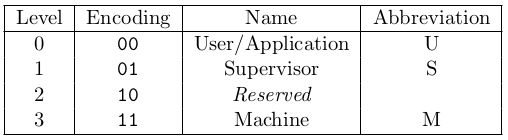
\includegraphics[width=0.5\linewidth]{Level.png}
		\bicaption{RISC-V的3个等级及其编码。\citep{privileged2017}表 1.1.}{RISC-V privilege levels and their encoding. Table 1.1 of \citep{privileged2017}.}
		\label{fig:mode}
	\end{figure}
	
	而这3个等级的2 bits编码均体现在特权指令的编码(用户态的指令不用这么编码是因为无论哪个等级都可以执行这些指令,而且省去这两位能够增加3倍的指令编码空间)和特权寄存器空间的编码。这样什么等级的指令执行在什么等级状态下处理器上,要修改什么等级的寄存器,非常的清晰明了。
	
	在三个等级中最为基础的就是Machine Level(以下简称M等级)。而M等级中基础的控制寄存器其实基本上和MIPS CP0寄存器是一一对应的。列举见表\ref{tab:sampleofCSR}:
	\begin{table}[!htbp]
		\bicaption{与MIPS CP0寄存器功能类似的CSR列表。}{The List of CSRs similar to MIPS CP0.}
		\label{tab:sampleofCSR}
		\centering
		\footnotesize% fontsize
		\setlength{\tabcolsep}{4pt}% column separation
		\renewcommand{\arraystretch}{1.2}%row space 
		\begin{tabular}{lll}
			\hline
			简称 & 全称 & 功能备注 \\%inserts table 
			%\cline{2-9}% partial hline from column i to column j
			\hline
			\tt mtvec    & \textit{Machine Trap Vector}       & 存储例外的跳转地址 \\
			\tt mepc     & \textit{Machine Exception PC}      & 存储例外发生的指令PC \\
			\tt mcause   & \textit{Machine Exception Cause}   & 指示例外发生的原因与类型 \\
			\tt mie      & \textit{Machine Interrupt Enable}  & 中断使能向量 \\
			\tt mip      & \textit{Machine Interrupt Pending} & 列举当前pending住的中断 \\
			\tt mtval    & \textit{Machine Trap Value} & 与MIPS中的BADADDR功能一致,存储例外访存地址 \\
			\tt mscratch & \textit{Machine Scratch}    & 一个指令长度的数据临时存储 \\
			\tt mstatus  & \textit{Machine Status}     & 与MIPS中的STATUS功能类似,存储处理器状态 \\
			\hline
		\end{tabular}
	\end{table}
	
	这里比较有特色的寄存器是mscratch。如果编写过或者看过MIPS上的操作系统内核,就会知道比如context switch和TLB的例外处理都需要用到K0和K1寄存器,这两个寄存器就是专门留给操作系统用于临时存储数据地址用的。虽然这样很高效,但是白白浪费了两个通用寄存器。另外一方面像context switch和TLB的例外处理是与M等级有关的,所以从设计的归类上来讲也应该归特权级别的寄存器管理而不是通用寄存器。这也是RISC-V更为干净的一种体现。
	
	在特权态中最为重要的一方面是内存管理,而一个最基本的考虑就是用户态不可信赖的程序要严格限制其只能访问到自己内存范围的内容。从RISC-V的手册\textit{The RISC-V Instruction Set Manual Volume II: Privileged Architecture}中,可以看得出其设计者在这方面下了很大的功夫。
	
	首先,RISC-V在M等级和User Level(以下简称U等级)之间设计了一种内存保护机制:Physical Memory Protection (PMP)。这样M等级就可以配置U等级程序能够访问的内存区域以及访问的权限。
	\begin{figure}[!htbp]
		\centering
		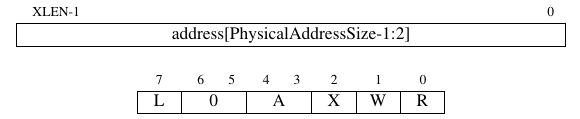
\includegraphics[width=0.7\linewidth]{PMP.png}
		\bicaption{PMP地址和配置寄存器。地址寄存器右移了2,如果物理地址比XLEN-1,那么高位填0. R, W和X域授权读,写,执行权限。A域设置PMP模式,L域锁住对应的PMP地址寄存器。\citep{Patterson:2017:RRO:3202479}图 10.7.}{A PMP address and configuration register. The address register is right-shifted by 2, and if physical addresses are less than XLEN-2 bits wide, the upper bits are zeros. The R, W, and X fields grant read, write, and execute permissions. The A field sets the PMP mode, and the L field locks the PMP and corresponding address registers. Figure 10.7 of \citep{Patterson:2017:RRO:3202479}.}
		\label{fig:pmp}
	\end{figure}
	上图\ref{fig:pmp}上半部分是PMP地址寄存器, 一般处理器会实现8-16个这样的寄存器;下半部分是PMP配置寄存器,为8-bit向量存储在pmpcfg的CSR寄存器里,负责授权或者禁止读、写、执行权限。当处理器在U-mode试图想要取指或者执行访存请求时,其地址将会被和PMP地址寄存器进行比较,如果地址大于等于$ i $号PMP而小于$ i+1 $号PMP。那么$ i+1 $号的PMP配置寄存器将会规定访问内存的模式,如果实际的访问方式逾越了配置寄存器里规定的权限,就会引发例外\citep{Patterson:2017:RRO:3202479}。
	
	对于嵌入式系统,PMP机制能够非常有效的对内存实行保护。但是其有两个缺点使之不适合更为复杂的系统和通用计算,分别是:
	\begin{enumerate}[label=(\alph*)]
		\item 只支持最多16个内存区域,不具备扩展性。
		\item 这些区域都是连续的,有点像操作系统早期的\textbf{段}的概念,所以对内存的细粒度的片段化支持不好。
	\end{enumerate}
	
	所以RISC-V的ISA必须支持基于页的虚拟内存机制。而这个特征直接主导了介于M等级和U等级中间的等级 --- supervisor mode(以下简称为S等级)的产生。
	
	但是引入S等级又会产生一个问题。RISC-V中所有的例外都是要将处理器的控制权转移到M等级的例外处理程序。但是大多数的Unix系统的系统调用包括例外是陷入系统内核,而系统内核又是运行在S等级的。如果先由系统将用户进程切换到内核,然后再由CPU硬件将内核S等级切换到M等级处理,最后M等级要重新路由到S等级,交给系统内核去退出系统调用\citep{Patterson:2017:RRO:3202479},这样效率就会大大降低。所以RISC-V提供了例外授权机制(exception delegation mechanism),这样中断和同步例外就能旁路到M等级,选择性的授权给S等级。而CSR寄存器 {\tt mideleg }(Machine Interrupt Delegation)和{\tt medeleg }(Machine Exception  Delegation) 正是这个机制的载体。对应于{\tt mip }和 {\tt mie }寄存器的exception code,举例来说,{\tt mideleg[5]} 对应于S等级的时钟中断,如果被置上,S等级的时钟中断将会把控制权转移到S等级的exception handler上而不是M等级的exception handler;同样,如果{\tt mideleg[15]}被置上,则会将store page faults授权给S等级来处理\citep{Patterson:2017:RRO:3202479}。不过需要注意的是,在某等级发生的例外永远不会转移控制权给更低的等级,具体来说就是在M等级发生的例外就只能M等级来处理;S等级发生的例外可能由M等级或者S等级来处理,取决于delegation的配置,但永远不会是U等级\cite{Patterson:2017:RRO:3202479}。
	
	RISC-V的分页方案命名方式为\textbf{SvX},比如32位的虚拟地址是\textbf{Sv32}, 其支持4GiB的虚拟地址,有两级页表,分别是$ 2^{10} $个 4MiB的页表,每个页表又有$ 2^{10} $个4KiB的基页。下图\ref{fig:SvX}是\textbf{Sv32}和\textbf{Sv39}的页表项(PTE):
	\begin{figure}[!htbp]
		\centering
		\begin{subfigure}[b]{0.7\textwidth}
			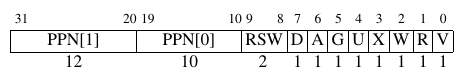
\includegraphics[width=\textwidth]{Sv32.png}
			\caption{}
		\end{subfigure}%
		
		\begin{subfigure}[b]{\textwidth}
			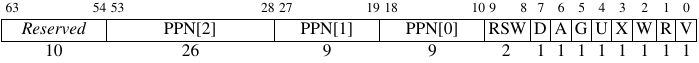
\includegraphics[width=\textwidth]{Sv39.png}
			\caption{}
		\end{subfigure}%
		\bicaption{RISC-V分页。\citep{Patterson:2017:RRO:3202479}图10.10和10.11. (a)RV32 Sv32页表项,(b)RV64 Sv39页表项。}
		{RISC-V SvX. Figure 10.10 and 10.11 of \citep{Patterson:2017:RRO:3202479}. (a)An RV32 Sv32 page-table entry(PTE), (b)An RV64 Sv39 page-table entry(PTE).}
		\label{fig:SvX}
	\end{figure}
	\textbf{Sv39}是$ 2^9\times 2^9\times 2^9 \times 2^{12} $的模式,是3级页表。如果物理地址比$ 2^{39} $还要大,RISC-V还提供了4级页表的\textbf{Sv48}方案。
	
	S等级用satp (Supervisor Address Translation and Protection)控制和状态寄存器管理分页系统,如下图\ref{fig:satp}:
	\begin{figure}[!htbp]
		\centering
		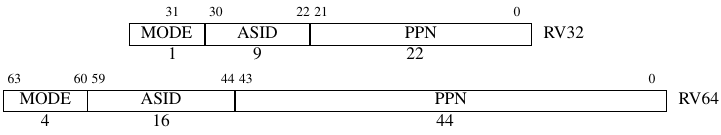
\includegraphics[width=0.7\linewidth]{satp.png}
		\bicaption{satp控制和状态寄存器 \citep{Patterson:2017:RRO:3202479}表 10.12.}{The satp CSR. Figure 10.12 of \citep{Patterson:2017:RRO:3202479}.}
		\label{fig:satp}
	\end{figure}
	在处理器进入S等级之前,M等级首先会写0到satp寄存器,禁止分页;然后等到进入S等级在初始化页表之后,处于S级内核就可以开始对satp寄存器进行操作来对内存进行分配了。
\end{enumerate}

\subsection{Verilog和Chisel}

设计的实现是将抽象的逻辑层面想法概念用具体的语言严谨地描述出来,同样,设计处理器这样的硬件需要硬件的描述语言。当今主流的描述语言仍是90年代开发的Verilog。该语言设计参考的是C语言,最开始设计出来用作电路功能的仿真,因而有很多语法只适用于软件的仿真,不能作为物理电路的综合布局布线。可被综合的最常用的语句是组合逻辑的assign语句块和时序逻辑的同步always语句块。事实上这两种语句组合就能够满足绝大多数的电路设计的需求,其中就包括双发射乱序处理器。但是就像能够描述所有软件程序的汇编语言一样,Verilog的抽象等级太低,细节太多,描述电路的能力先天不足,主要体现在:
\begin{enumerate}[label=(\alph*)]
	\item 语句的逻辑集成度不高,时常一个简单的逻辑代码量却不少。
	\item 变量名、函数名、参数名的管理机制原始落后,甚至都没有像C语言的struct结构体这种聚合化的设计。代码量大时,各个符号名称的关联往往复杂而混乱。
	\item 常用的简单逻辑代码复用度不高,代码复用基本上只能用Module这样一种单一的写法,容易冗余。
	\item 对多维的向量数组描述和聚合化操作支持不足。
	\item 没有成熟的类型系统,无论是Reg还是Wire都是对物理信号的刻画描述,粒度太小。
	\item 容易一不小心出现组合环,现有的编译器有很难跟踪。
	\item 要实例化不同参数的同一模块,只能一个个实例,做不到参数的数组化。
\end{enumerate}

设想原本逻辑已经复杂不堪的双发射乱序处理器采用Verilog来描述,又会因为语言层面的弱势,使得实现起来异常的繁琐,复杂度得不到有效地控制。对这样的大工程的搭建、调试以及持续的优化、增量式演进都带来不小的挑战。

硬件工程师迫切需要一个更为高级的语言来解决上述Verilog种种缺陷,这就是Chisel。

Chisel没有那么神秘,并不是变革性的另一套硬件描述,而是包装在verilog之上具有面向对象和函数化编程特性的Scala脚本语言,是一种以Verilog中上述两种语句为基本块的更上一层的抽象。多一层的抽象就是为了解决Verilog表示能力不足的缺陷。比如Chisel支持面向对象里的类和对象、接口以及多态与继承的特性,可以很好地复用代码,有条理地管理变量名、方法名和参数名;另外函数式的编程可以用来很便捷的描述简单的电路逻辑,增强对多维数组操作的支持。对应的,Chisel的编译器主要工作就是将抽象的Scala代码转化为低级的Verilog,而且是完全可以被综合和物理实现的Verilog (所以是否是可综合的电路根本不需要顾虑)。类似于JAVA编译器将JAVA编译成汇编代码。

Chisel和JAVA都是强类型的语言(Chisel的类型继承关系如图\ref{fig:type} (\url{https://chisel.eecs.berkeley.edu/2.2.0/manual.html}),在编译的时候会做类型检查,从而避免很多因为类型不当导致的逻辑错误。而Verilog和汇编都是没有类型的概念的,一个32位的逻辑寄存器,汇编可以任意的操作而不用在乎这个寄存器代表的是整型还是字符型,同样,Verilog对一个32bit的Wire和Reg向量也可以任意操作。正是因为这种毫无约束的操作,使得用汇编或者Verilog编程都会比Chisel或者JAVA来得繁琐而易出错。但是略显不同的是,一个初学者可以在不知道汇编语言的情况下就能够掌握JAVA语言这样的抽象等级高的语言,但是却不能在没有熟练运用Verilog中的两个基本语句的前提下掌握Chisel。换言之JAVA对于汇编的抽象是彻底的,而Chisel对于Verilog的抽象是不彻底的,所以Chisel适用于有一定硬件设计工程经验的人,而不适用于上手设计电路的初学者。
\begin{figure}[!htbp]
	\centering
	\begin{subfigure}[b]{0.35\textwidth}
		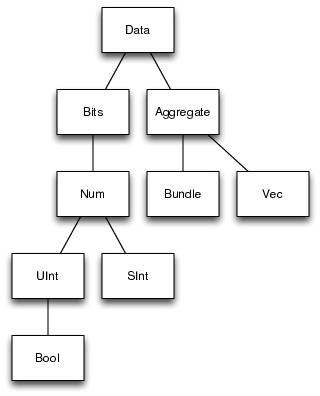
\includegraphics[width=\textwidth]{type-hierarchy.png}
		\caption{}
		\label{fig:type}
	\end{subfigure}%
	~%add desired spacing
	\begin{subfigure}[b]{0.65\textwidth}
		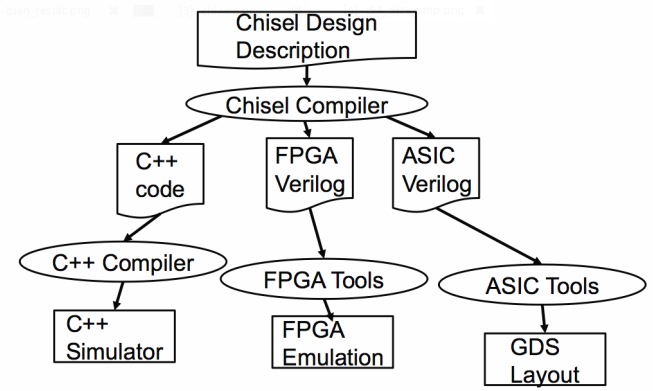
\includegraphics[width=\textwidth]{Chisel_data_flow.png}
		\caption{}
		\label{fig:design_flow}
	\end{subfigure}
	\bicaption{Chisel的类型层次结构和设计流。(a) Chisel类型系统,(b) 基于Chisel的设计流程框图。\citep{lab1}图 1.}{Chisel type hierarchy and Chisel Design Flow. (a) Chisel type hierarchy, (b) Chisel Design Flow. Figure 1 of \citep{lab1}.}
	\label{fig:chisel_into}
\end{figure}

从Chisel设计流程框图\ref{fig:design_flow}可以发现,首先Chisel通过编译器不仅能够编译成Verilog,还能编译成C++代码再通过C++的编译器得到C++的模拟器。工程实践证明,C++模拟器仿速度非常快,跑500遍dhrystone仅仅需要1秒。其次Chisel编译器可以针对不同的硬件平台编译采用不同的优化。甚至得到的电路时序比人写的Verilog对应的电路还要好。

但是电路描述高级语言化首先需要克服电路方面特有的两大障碍:
\begin{enumerate}[label=(\arabic*)]
	\item 时序逻辑高级语言应该如何描述?
	\item 随着语言的高级化,会不会使得电路的编写模糊化,使得所写的电路很难对应到实际的物理电路上,就像高级语言对垃圾回收做了透明化一样。这恰恰是硬件的工程师所不愿意看到的,因为电路设计要了解电路的所有实现细节。
\end{enumerate}

那么Chisel是如何成果性地打消上述的两个障碍和顾虑的呢?那就要看Chisel是如何进行抽象的。
\begin{enumerate}[label=(\alph*)]
	\item 组合电路的对应于Verilog中的Wire,赋值用assign语句,也可以直接在Wire型变量定义的时候赋值。而Chisel首先用的就是两类最基本的数据类型来描述,分别是UInt和Bool。Bool只是为了强调变量是1 bit的代表真假布尔逻辑的变量。而Wire型变量的赋值有两种形式:
	\begin{itemize}
		\item 初始定义的 \textbf{=} 运算符 
		\begin{scala} 
			val pc = Wire(UInt())
		\end{scala}
		
		如上并不是真正的赋值,而是类型的申明。UInt的括号中可以传入位宽的参数,如果省略,Chisel会在编译的时候自动在以后的真正赋值中推导出来,所以还是非常人性化的。
		\item 因为val在Scala中是不可变量,也就是变量名指针所指的对象不能更改,所以chisel中引入\textbf{:=}运算符来进行再赋值。
		\begin{scala} 
			pc := pcReg + 4.U 
		\end{scala}		
	\end{itemize}
	\item 时序电路对应于Verilog中的reg,赋值需要用到always语句。而在Chisel对其进行了抽象,首先它没有具体的类型,是一个Reg的元器件。其次这个元器件有两端 --- input和output。而output可以理解为input信号延迟一周期的副本。严格来讲,Reg型变量的类型可以定义为input端所连的变量的类型,在reg类型变量的定义中还可以指明reset的初始值。如下例:
	\begin{scala}
		val pcReg = Reg(next = pcNext, init = 0.U(32.W))
	\end{scala}
	在当前的版本的Chisel中,时钟和复位是全局信号,是隐式申明的\citep{chisel2017}。
	这样Reg型的变量的更新可以做到简单一行的赋值代码,和组合逻辑Wire型变量一样使用\textbf{:=}运算符。
	\item 由于赋值运算符的统一,Chisel对于wire类型和reg类型的变量统一抽象为了电路上的节点(node)。整个电路图就是由node组成的图。具体来讲,如果是纯组合逻辑,那么这个图就是有向无环图,所以Chisel是可以对于设计中出现的组合环会进行非常精确的报错,指出相同的开始节点和结束节点,从而规避了仿真中出现的奇怪的现象。唯一存在有环的情况是时序电路。而且依据这个图,可以用verilator工具生成高速的C++的simulator\citep{chisel2017}。
	\item 变量统一抽象为电路节点反过来将\textbf{:=}运算符的意义统一了 --- 将右手表达式代表的节点组合逻辑连线到左手变量代表的目的节点上。但是略有差异而且需要注意的是,如果涉及到Reg型变量\textit{x},因其具有两端,若\textit{x}出现在右手表达式,用的是output端;若\textit{x}出现在左手表达式,用的是input端\citep{chisel2017}。
	
	\item 有了基础的抽象,Chisel可以在其上利用面向对象的方法和继承的手法自定义构建更为大型,更为抽象的数据结构。
	\item 类比在Verilog对于模块的刻画用了module的写法,Chisel采用用户自定义类去继承称为Module的父类的写法,并且对于模块的接口,还定义了一个IO的类。如下例\citep{chisel2017}:
	\begin{scala}
		class Mux2 extends Module {
			val io = IO(new Bundle{
				val sel = Input(UInt(1.W))
				val in0 = Input(UInt(1.W))
				val in1 = Input(UInt(1.W))
				val out = Output(UInt(1.W))
			})
			io.out := (io.sel & io.in1) | (~io.sel & io.in0)
		}
	\end{scala}
	这里的Bundle是一个Chisel里的基类,类似于C里面的\textit{Struct}。但是如上述例子所展示的,可以不需要对这个结构体预先定义而直接新建一个匿名的结构体,然后作为参数传入IO的构造方法中,最后将其赋值给IO。这种写法相比于Verilog里最大的好处在于在Module的内部的逻辑中,Chisel的代码更加清晰。端口因为都带有\textit{io.}的前缀,引用或者赋值一目了然。这样增加了代码的可读性。
\end{enumerate}

经过上面的分析,Chisel语言依旧能够呈现统一时钟复位电路的所有细节。如果尚有缺点,也是因为目前屏蔽了clock和reset,默认为统一时钟同步复位,还不支持异步电路。这个在Chisel的文档里也给出了解释:纵然有交叉时钟的设计需求,但是现代设计方法中也是在每一个同步的电路岛屿中开发与验证的\citep{chisel2017}。

下面用三个例子来展示Chisel在电路设计的简便之处:
\begin{enumerate}[label=(\arabic*)]
	\item 下面代码\citep{chisel2017}灵活运用了面向对象和可配置参数化函数(类似于C++的template)的语言特性。首先是通过面向对象的继承来充分复用已有的代码逻辑,其次不同功能的Filter利用$\lambda$-函数作为参数传入,来充分复用不同Filter相同逻辑的部分,与此同时并没有掩盖电路的细节。
	\begin{scala}
		abstract class Filter[T <: Data](dtype: T) extends Module {
			val io = IO(new Bundle {
				val in = Input(Valid(dtype))
				val out = Output(Valid(dtype))
			})
		}
		class PredicateFilter[T <: Data](dtype: T, f: T => Bool) extends Filter(dtype) {
			io.out.valid := io.in.valid && f(io.in.bits)
			io.out.bits  := io.in.bits
		}
		object SingleFilter {
			def apply[T <: UInt](dtype: T) = 
			Module(new PredicateFilter(dtype, (x: T) => x <= 9.U))
		}
		object EvenFilter {
			def apply[T <: UInt](dtype: T) = 
			Module(new PredicateFilter(dtype, (x: T) => x(0).toBool))
		}
		class SingleEvenFilter[T <: UInt](dtype: T) extends Filter(dtype) {
			val single = SingleFilter(dtype)
			val even   = EvenFilter(dtype)
			single.io.in  := io.in
			even.io.in    := single.io.out
			io.out        := even.io.out
		}
	\end{scala}
	
	\item 拷贝于毕业设计代码中的顶层文件。可以看到其中颇具特点的运算符\textbf{<>}(在Chisel的术语里叫做\textit{Bulk Connections}),大大简化了模块实例化后互相连线的逻辑,相当于一些输入输出信号集合整体的连线。
	\begin{scala}
		class Core(implicit conf: CPUConfig) extends Module with BTBParams {
			val io = IO(new Bundle {
				val imem = new AxiIO(conf.xprlen)
				val dmem = new MemPortIo(conf.xprlen)
			})
			val frontEnd = Module(new FrontEnd)
			val backEnd  = Module(new BackEnd)
			frontEnd.io.mem  <> io.imem
			backEnd.io.mem   <> io.dmem
			frontEnd.io.back <> backEnd.io.front}
	\end{scala}
	
	\item 拷贝于毕业设计代码中的写回结果总线监听逻辑。发射队列有nEntry项,每一项存有一条待发射的指令,需要监听两个源操作数,写回总线结果对应于代码中的\textit{io.bypass}。下面短短几行的代码里就涵盖了将写回总线的寄存器地址和有效使能信号逐一与发射队列里的每一项待发射指令的每一个源操作数进行比对,判断是否成功监听的逻辑。Chisel对于数组聚合化操作的强大描述能力可见一斑。
	\begin{scala}
		for (i <- 0 until nEntry) {
			for (j <- 0 until 2) {
				inst_ctrl.snoop(i)(j) := issue.snoop(i)(j).valid ||
				io.bypass.map(b => 
				b.addr === issue.snoop(i)(j).addr && b.valid).reduce(_||_)
			}
		\end{scala}
		
	\end{enumerate}
	
	\subsection{RISC-V开源仓库}
	RISC-V近年的流行和其开源仓库是相辅相成的,目前在开源的工程下至较为成熟的处理器设计实现以及整套SoC的环境,上至各种软件栈一应俱全。使得大至一个国家如印度,中至一些企业组织如lowRISC,小至一个个独立的研究个体都愿意加入到RISV-C的开发中来。
	
	具体对设计影响较大的几个开源工程有开发语言Chisel,双发射乱序处理器BOOM及其设计文档和RISC-V整套在x86 host机上处理器设计的调试环境。
	
	\section{研究范围}
	
	一个人做出一个功能齐全,能够运行操作系统和整套软件栈的双发射乱序处理器,在半年时间内几乎是不可能完成的。所以研究的范围应该集中在乱序的调度,分支的预测以及取指部件的高效取指上,最后能够运行简单嵌入式程序来初步验证处理器正确性和评测性能即可。
	
	在摘要中已经提及了必要的简化方案,更具体的方案包括:不支持MMU以及分页机制;取指为了实现取指宽度大于1实现了icache并且对外是AXI接口,测试的时候带有随机的取指延迟;访存虽然支持访存延迟,但没有实现dcache,对外也不是AXI接口,访存过程几乎是一个周期的同步时序。
	